\section{Deployment and reproducibility}
\label{sec:deployment}

\subsection{The application}
One FastAPI~\cite{fastapi} backend serves two React applications (Figure~\ref{fig:screens}):
\begin{itemize}
  \item the \textbf{front office}, for customers and advisors: a help centre with semantic search, demo
        customers on real Olist orders, a live chat with the AI advisor (streamed word by word, with a
        ``behind the scenes'' trace of every agent, tool and policy section, then a satisfaction survey and the
        quality review), an advisor desk (queue, copilot drafts, autopilot), voice input through the browser's
        speech recognition, and a phone page;
  \item the \textbf{back office}, for managers: data and contracts, the forecast, the digital twin (a live floor
        that replays a simulated day contact by contact, and a scenario lab), the agent theatre, workforce
        planning, models and MLOps, the \textbf{AI monitoring} page (Section~\ref{sec:monitoring}), and a
        full-screen \textbf{live contact centre} (Figure~\ref{fig:centre}) where every move of the animated
        staff is a real event: a customer walks in (an AI customer, an existing customer or a new one with a
        new problem), the receptionist (Workforce agent) routes the chat, the advisor answers with tool badges
        in its speech bubbles, and the quality lead posts the score. Real chats from the portal or the phone
        appear there too, and each person can speak their lines aloud.
\end{itemize}

\begin{figure}[!htbp]
\centering
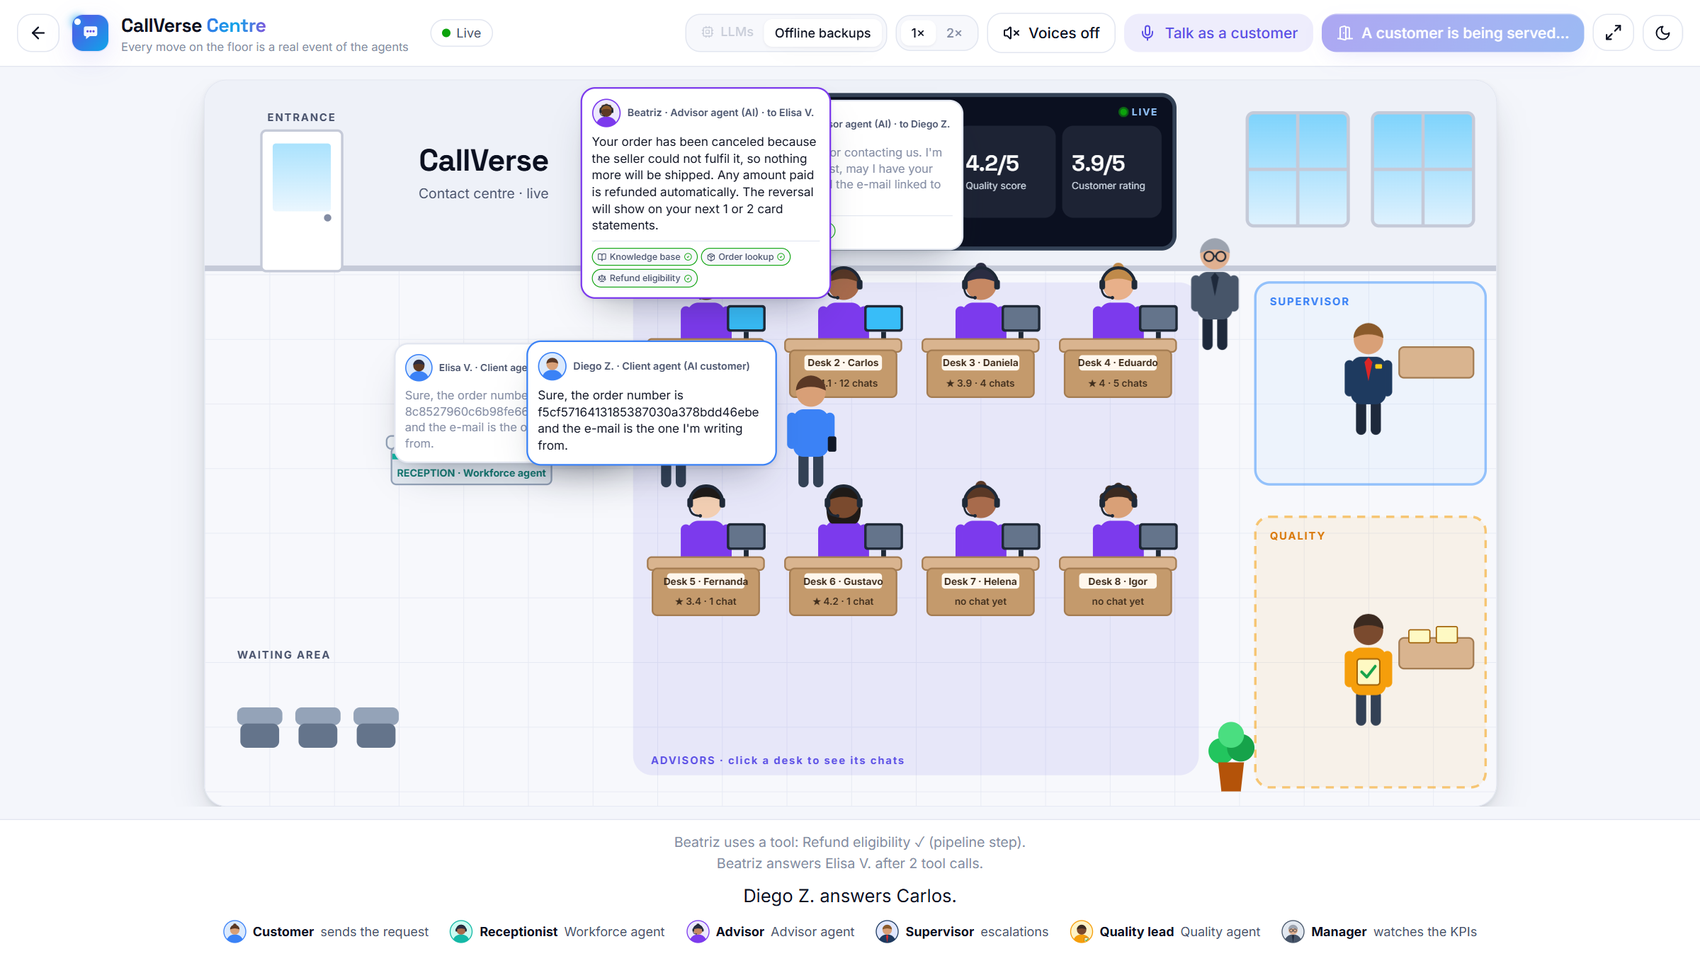
\includegraphics[width=\textwidth]{figures/screen_centre.png}
\caption{The live contact centre (back office, full screen), here with the offline templates. Two AI customers
were routed by the Workforce agent to desks 1 and 2. Beatriz's answer carries the badges of the tools behind it
(knowledge base, order lookup, refund eligibility); the footer narrates each real event, such as ``Beatriz uses
a tool: Refund eligibility (pipeline step)''.}
\label{fig:centre}
\end{figure}
The live chat and the contact centre use WebSockets. The API is documented with OpenAPI at \code{/docs}, and an
MCP server exposes the business tools to outside AI applications (stdio or \code{/mcp} over HTTP).

\begin{figure}[!htbp]
\centering
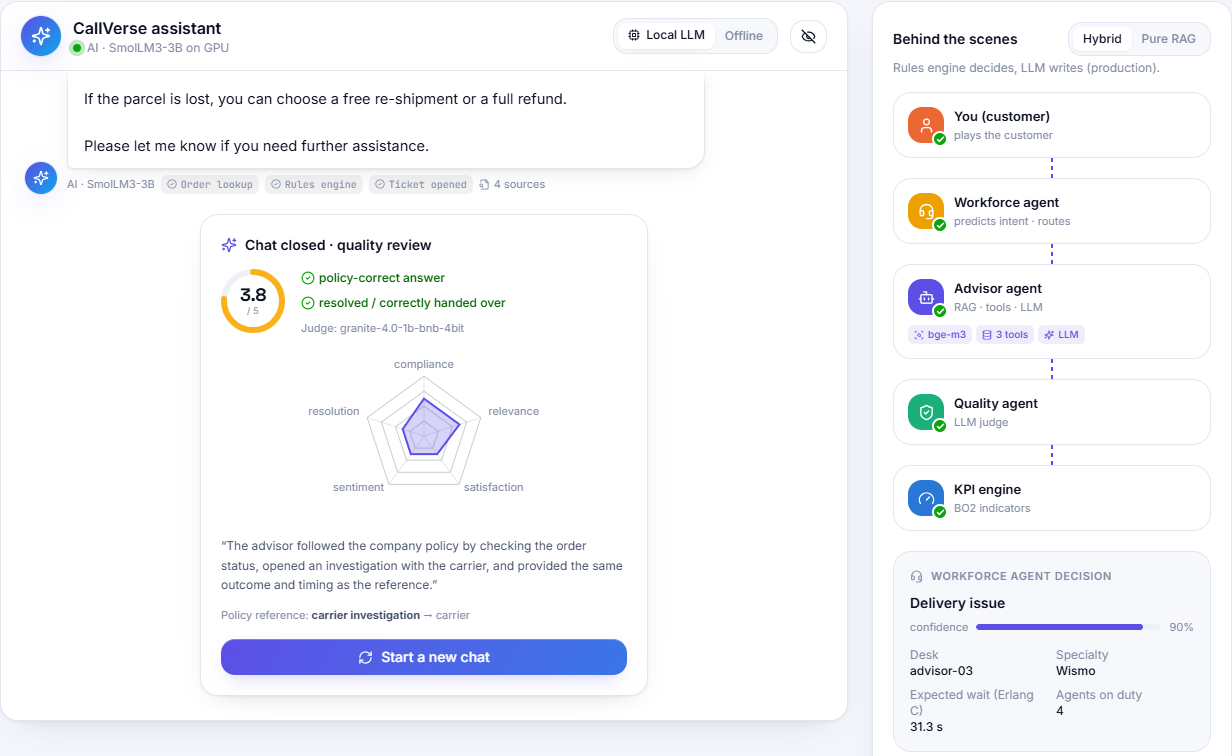
\includegraphics[width=0.53\textwidth]{figures/screen_chat_review.png}\hfill
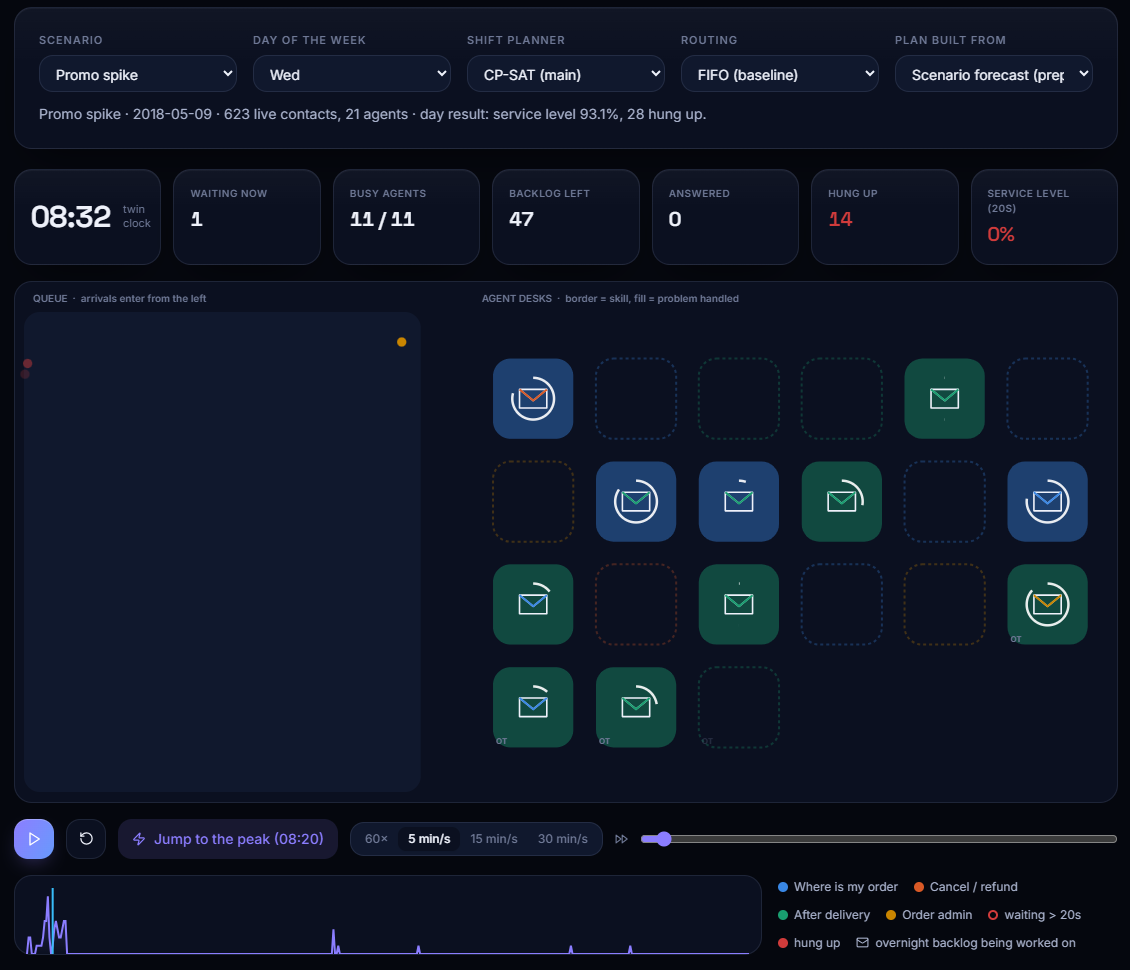
\includegraphics[width=0.44\textwidth]{figures/screen_twin_floor.png}
\caption{Left: the front office after a chat, with the quality review and the ``behind the scenes'' trace
(captured on 1 November 2026, in the local-model period). Right: the twin's live floor replaying a promotion
day with a CP-SAT plan.}
\label{fig:screens}
\end{figure}

\subsection{One container}
The whole application ships as \textbf{one Docker image}. A first stage builds the two React apps with Node; a
second stage installs the Python package on Python 3.12 and serves both apps from the API: the front office at
\code{/}, the back office at \code{/back-office/}, the API at \code{/api}, \code{/ws}, \code{/docs} and
\code{/mcp}. Three details make the image reproducible: the library versions are pinned to those of the
environment that trained the saved models (\code{space/constraints.txt}, 31 libraries, so the scikit-learn
classifier, the PPO policy and the MLflow database load unchanged); the bge-m3 model is downloaded at build time
and the build fails if it cannot load \emph{offline}; and the Linux builds of the JavaScript build tools are
added, because the lock file was produced on Windows. For local use, Docker Compose also runs MLflow with
PostgreSQL and an nginx front.

\subsection{Online deployment}
Our first target was Hugging Face Spaces, which used to host Docker apps for free. On 11 November 2026 the
platform answered that Docker Spaces now require a paid subscription (HTTP 402), so we deploy on
\textbf{Azure for Students}. Its credit-only subscriptions cannot run cloud image builds (ACR Tasks), and
pushing a 6 GB image over our connection would take hours. We therefore use a small Linux virtual machine
(Ubuntu 24.04, 2 vCPUs, 8 GB): \code{scripts/deploy\_azure.py} sends only a cleaned build folder (about 120 MB
compressed), the VM downloads the heavy parts and builds the image itself, and a Caddy container in front
obtains a free Let's Encrypt certificate. HTTPS is required for the microphone and for secure WebSockets.
The demo runs at \demourl.

Before anything leaves the laptop, the deployment script copies an \emph{allowlist} of files (never \code{.env},
keys or caches), deletes the customers we created while testing (our own names) from the copied database and
compacts it, so the deleted rows cannot be recovered, leaves out our live chat transcripts, keeps only the
numbers of the LLM trace, and stops if it finds a secret or one of the removed names. The OpenRouter key goes to
the VM through SSH input into a file only the service user can read. The public demo has no login, and visitor
data is reset at each deployment: it is a demonstration, not a production service.

\subsection{Reproducibility and code quality}
\begin{itemize}
  \item \textbf{One command per stage}: \code{callverse all} runs the whole pipeline (data, contracts,
        forecast, RL training, experiments, scorecard); \code{callverse evaluate} re-runs every experiment of
        Section~\ref{sec:experiments}. Notebooks are executed headless and their outputs archived.
  \item \textbf{Fixed randomness}: seeds live in \code{configs/}; experiments use common random numbers; CP-SAT runs
        on one thread so that the roster does not change between runs.
  \item \textbf{Pinned models and versions}: Hugging Face commits are recorded (\code{llm\_models.lock.json}),
        LLM answers are cached, and library versions are pinned for deployment.
  \item \textbf{Tracking}: MLflow records the parameters, metrics and artefacts of the forecast, RL and
        evaluation runs; every LLM call is traced.
  \item \textbf{Tests and checks}: 200 automated tests (unit, smoke and integration; they cover every layer,
        including live WebSocket sessions, the contact-centre hub and the serving of the built apps), the
        \code{ruff} linter,
        six import contracts for the layered architecture, and a GitHub Actions workflow that runs them and
        type-checks and builds both web apps.
  \item \textbf{Documentation}: the README (installation, execution, structure), a step-by-step run guide, the
        data reports of every phase, and the experiment protocol.
\end{itemize}
